\chapter{Экспериментальная оценка} \label{ch6}

В данной главе представлены результаты сравнительного эксперимента. 
В параграфе~\ref{ch6:sec1} описаны наборы данных и параметры эксперимента. 
В параграфе~\ref{ch6:sec3} приведены результаты на наборе данных BigFaultMatrix. 
В параграфе~\ref{ch6:sec4} приведены результаты на проектах Defects4J. 
В параграфе~\ref{ch6:sec5} выполнен анализ результатов.

\section{Наборы данных и параметры эксперимента} \label{ch6:sec1}

В эксперименте используются два публичных набора данных.

\textbf{BigFaultMatrix}~\cite{paygude2020} --- бинарная матрица размером $1000 \times 38$, 
где строки соответствуют тестовым случаям, столбцы --- дефектам. Для расширения бенчмарка 
дополнительно генерируются три вариации путем случайного инвертирования 10\%, 20\% и 30\% ячеек матрицы.

\textbf{Defects4J}~\cite{mahdieh2021} --- репозиторий реальных 
дефектов в Java-проектах с открытым исходным кодом. Используются даные репозитория предоставляющего 
матрицы покрытия методов, карты убитых мутантов и оценки вероятности дефектов на основе CIA-анализа.

В эксперименте задействованы 7 проектов, характеристики которых приведены в таблице~\ref{tab:datasets}.

\begin{table}[h]
\caption{Характеристики проектов Defects4J}
\label{tab:datasets}
\begin{tabularx}{\textwidth}{|X|c|c|}
\hline
Проект & Тестов & Мутантов \\
\hline
Jsoup/93            & 690  & 30   \\
Csv/16              & 284  & 99   \\
JacksonDatabind/112 & 36   & 37   \\
Time/27             & 3768 & 828  \\
Codec/18            & 834  & 26   \\
JacksonCore/26      & 108  & 2002 \\
Lang/65             & 1609 & 351  \\
\hline
\end{tabularx}
\end{table}

\newpage
Сравниваются четыре алгоритма:
\begin{itemize}
    \item \textbf{Random} --- случайная перестановка тестов, 
    нижняя граница сравнения. Результат усредняется по 5 прогонам.
    \item \textbf{Additional} --- жадный алгоритм дополнительного 
    покрытия, классический baseline для TCP.
    \item \textbf{GA-Base} --- генетический алгоритм с фитнесс-функцией 
    только по покрытию ($w_c = 1{,}0$, $w_r = 0$, $w_d = 0$).
    \item \textbf{GA-FP+Div} --- предлагаемый метод с 
    фитнесс-функцией по покрытию, вероятности дефектов и 
    структурному разнообразию ($w_c = 0{,}4$, $w_r = 0{,}4$, 
    $w_d = 0{,}2$).
\end{itemize}


Параметры генетических алгоритмов: размер популяции $N = 100$, вероятность кроссовера $p_c = 0{,}8$, 
вероятность мутации $p_m = 0{,}2$, число поколений $$G = \max(50,\ 
\lfloor\log_2(n)\rfloor \cdot 10)$$. 
Эксперименты проводились на фиксированном зерне генератора случайных чисел для воспроизводимости результатов.

\section{Анализ чувствительности весов} \label{ch6:sec2}

Для обоснования выбора весов фитнесс-функции проведён анализ 
чувствительности: перебраны все комбинации $w_c$, $w_r$, $w_d$ 
с шагом $0{,}2$ при условии $w_c + w_r + w_d = 1$. Для каждой 
конфигурации вычислялся средний APFD по всем 7 проектам Defects4J.

Результаты показали что алгоритм устойчив к выбору весов: 
конфигурации с $w_r \geq 0{,}2$ дают средний APFD в диапазоне 
$[0{,}96;\ 0{,}98]$. Конфигурации без компоненты вероятности 
дефектов ($w_r = 0$) значительно уступают --- средний APFD 
составляет $0{,}929$, что подтверждает вклад CIA-данных в 
качество приоритизации.

Оптимальная конфигурация $w_c = 0{,}2$, $w_r = 0{,}6$, 
$w_d = 0{,}2$ обеспечивает средний APFD = $0{,}9785$ и принята 
в настоящей работе как основная.

\section{Результаты на BigFaultMatrix} \label{ch6:sec3}
Результаты эксперимента на четырёх вариациях BigFaultMatrix 
приведены в таблице~\ref{tab:bfm} и на рисунке~\ref{fig:bfm}.

\begin{table}[h]
\caption{Результаты на BigFaultMatrix (APFD)}
\label{tab:bfm}
\begin{tabularx}{\textwidth}{|X|c|c|c|c|}
\hline
Вариация & Random & Additional & GA-Base & GA-FP+Div \\
\hline
Оригинал & 0{,}9230 & \textbf{0{,}9987} & 0{,}9168 & 0{,}9590 \\
Flip 10\% & 0{,}9925 & \textbf{0{,}9983} & 0{,}9914 & 0{,}9973 \\
Flip 20\% & 0{,}9962 & \textbf{0{,}9988} & 0{,}9962 & 0{,}9984 \\
Flip 30\% & 0{,}9977 & \textbf{0{,}9989} & 0{,}9967 & 0{,}9987 \\
\hline
\end{tabularx}
\end{table}

\begin{figure}[h]
\centering
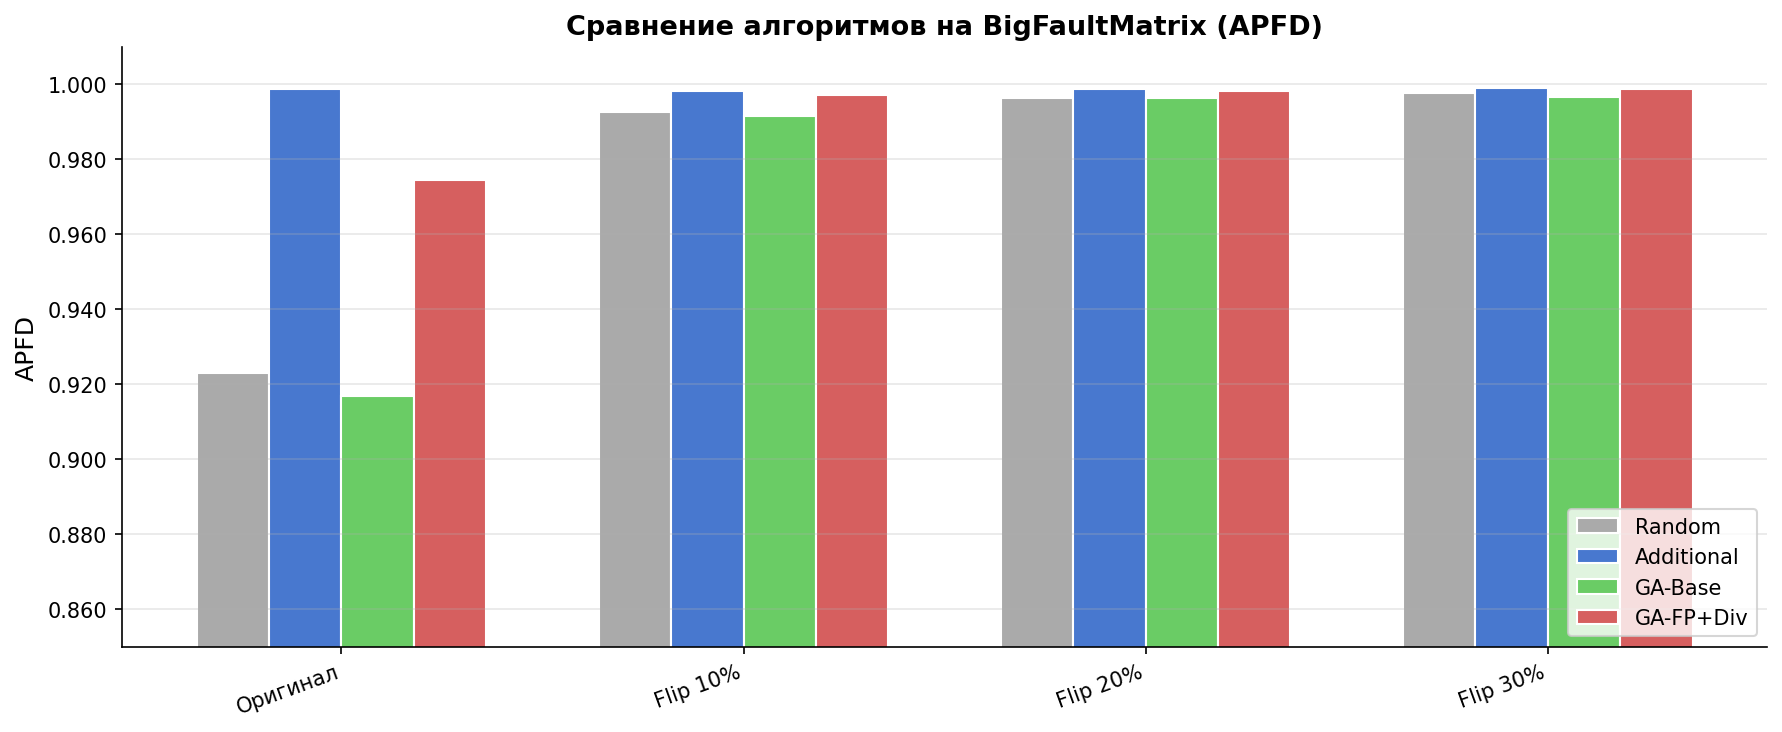
\includegraphics[width=\textwidth]{my_folder/images/bfm_apfd.png}
\caption{Сравнение алгоритмов на BigFaultMatrix по метрике APFD}
\label{fig:bfm}
\end{figure}

На данном наборе данных алгоритм Additional показывает наилучшие результаты во всех четырёх вариациях. 
Это объясняется структурой BigFaultMatrix: покрытие тестов непосредственно соответствует обнаружению 
дефектов, что делает жадную стратегию близкой к оптимальной. Генетические алгоритмы уступают Additional,
поскольку сигнал вероятности дефектов в данном формате слаб.

\section{Результаты на Defects4J} \label{ch6:sec4}

Результаты эксперимента на проектах Defects4J приведены в 
таблице~\ref{tab:d4j} и на рисунке~\ref{fig:d4j}.


\begin{table}[h]
\caption{Результаты на проектах Defects4J (APFD)}
\label{tab:d4j}
\begin{tabularx}{\textwidth}{|X|c|c|c|c|}
\hline
Проект & Random & Additional & GA-Base & GA-FP+Div \\
\hline
Jsoup/93            & 0{,}9115 & 0{,}9811 & 0{,}9936 & \textbf{0{,}9993} \\
Csv/16              & 0{,}9915 & 0{,}9958 & 0{,}9925 & \textbf{0{,}9982} \\
JacksonDatabind/112 & 0{,}8945 & 0{,}8803 & 0{,}8697 & \textbf{0{,}9163} \\
Time/27             & 0{,}9876 & \textbf{0{,}9965} & 0{,}9885 & 0{,}9928 \\
Codec/18            & 0{,}9373 & 0{,}9749 & 0{,}9782 & \textbf{0{,}9950} \\
JacksonCore/26      & 0{,}8643 & \textbf{0{,}9623} & 0{,}8854 & 0{,}9480 \\
Lang/65             & 0{,}9342 & 0{,}9842 & 0{,}9674 & \textbf{0{,}9997} \\
\hline
\end{tabularx}
\end{table}

\begin{figure}[h]
\centering
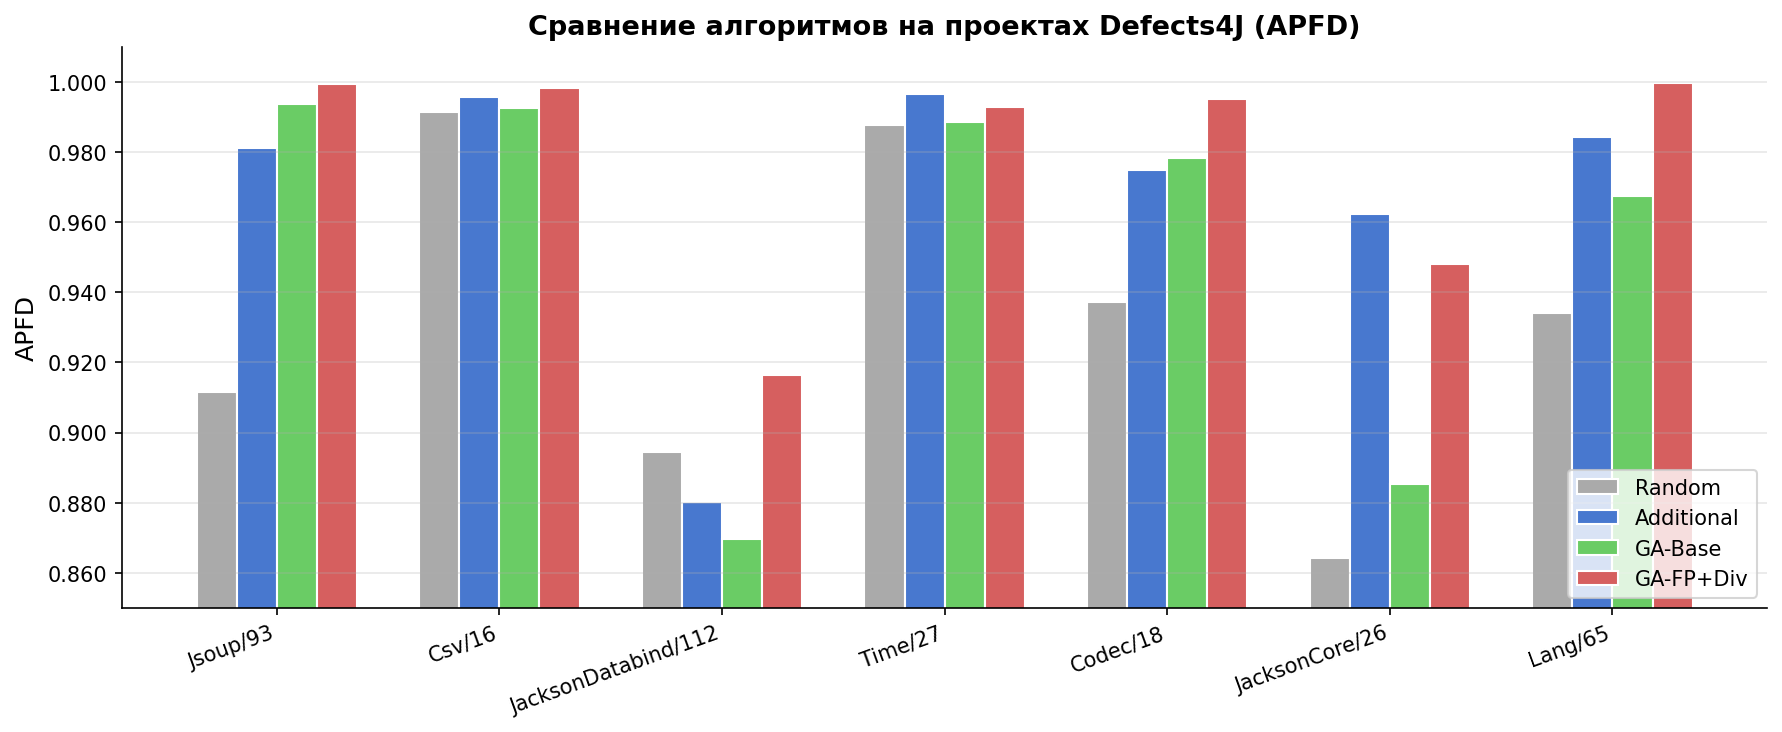
\includegraphics[width=\textwidth]{my_folder/images/defects4j_apfd.png}
\caption{Сравнение алгоритмов на проектах Defects4J по метрике APFD}
\label{fig:d4j}
\end{figure}

\newpage
\section{Анализ результатов} \label{ch6:sec5}

На проектах Defects4J алгоритм GA-FP+Div показывает наилучшие результаты на 5 из 7 проектов. 
На проектах Time/27 и JacksonCore/26 лучшим оказывается Additional. 
Это объясняется малым числом методов с ненулевой вероятностью дефектов по данным CIA-анализа: для 
Time/27 и JacksonCore/26 CIA предоставляет слабый сигнал, что снижает вклад компоненты вероятности 
дефектов в фитнесс-функцию.

На проектах с богатыми CIA-данными (Codec/18, Lang/65, Jsoup/93) преимущество GA-FP+Div наиболее выражено. 
Например, на Codec/18 GA-FP+Div достигает APFD = 0{,}9994, превосходя Additional (0{,}9749) на 2{,}5 
процентных пункта.

Алгоритм GA-Base уступает GA-FP+Div на всех проектах Defects4J, что подтверждает эффективность 
добавления компонент вероятности дефектов и структурного разнообразия в фитнесс-функцию.

Таким образом, GA-FP+Div демонстрирует устойчивое преимущество над базовым генетическим алгоритмом, 
а его эффективность относительно жадного алгоритма определяется качеством CIA-данных для конкретного проекта.